% !TEX root =  ../Report.tex

\chapter{Software Deliverable}
\label{sec:chap-4}
In the current section, we give an extensive overview of the
software tool we developed to help with the our theory crafting.
Core idea is to be able to draw \textit{PureCircuit} gadgets,
verify correctness and find solutions. We split
this chapter giving an overview on the tooling we used,
the architecture of the software
the algorihtms we deployed for solutions finding.


\section{Tooling Selection}

\subsection{Rust Programming Language} The development language used for is \texttt{Rust} \footnote{https://www.rust-lang.org/}.
Rust is a systems-level compiled programming language that can achieve high speeds due to
its low-level compilation, while maintaining memory safety. The key reasons,
for the specific language of choice is its speed as well as having an advanced
algebraic type system.

\subsection{Bevy and the ECS architecture} \texttt{Bevy} \footnote{https://bevy.org/} is a \texttt{Rust} library,
primarily used for game development. It uses the Entity-Component-System architecture
where entities with varying components exist in world state. Each \textit{entity}
interacts with each other based on systems. A visual reference is provided in the
figure \ref{fig:chap-4:ecs-example}. The idea is that we are able to decouple
the logic from entities to their individual components and express
more intricate relations.

\begin{figure}[h!]
    \centering
    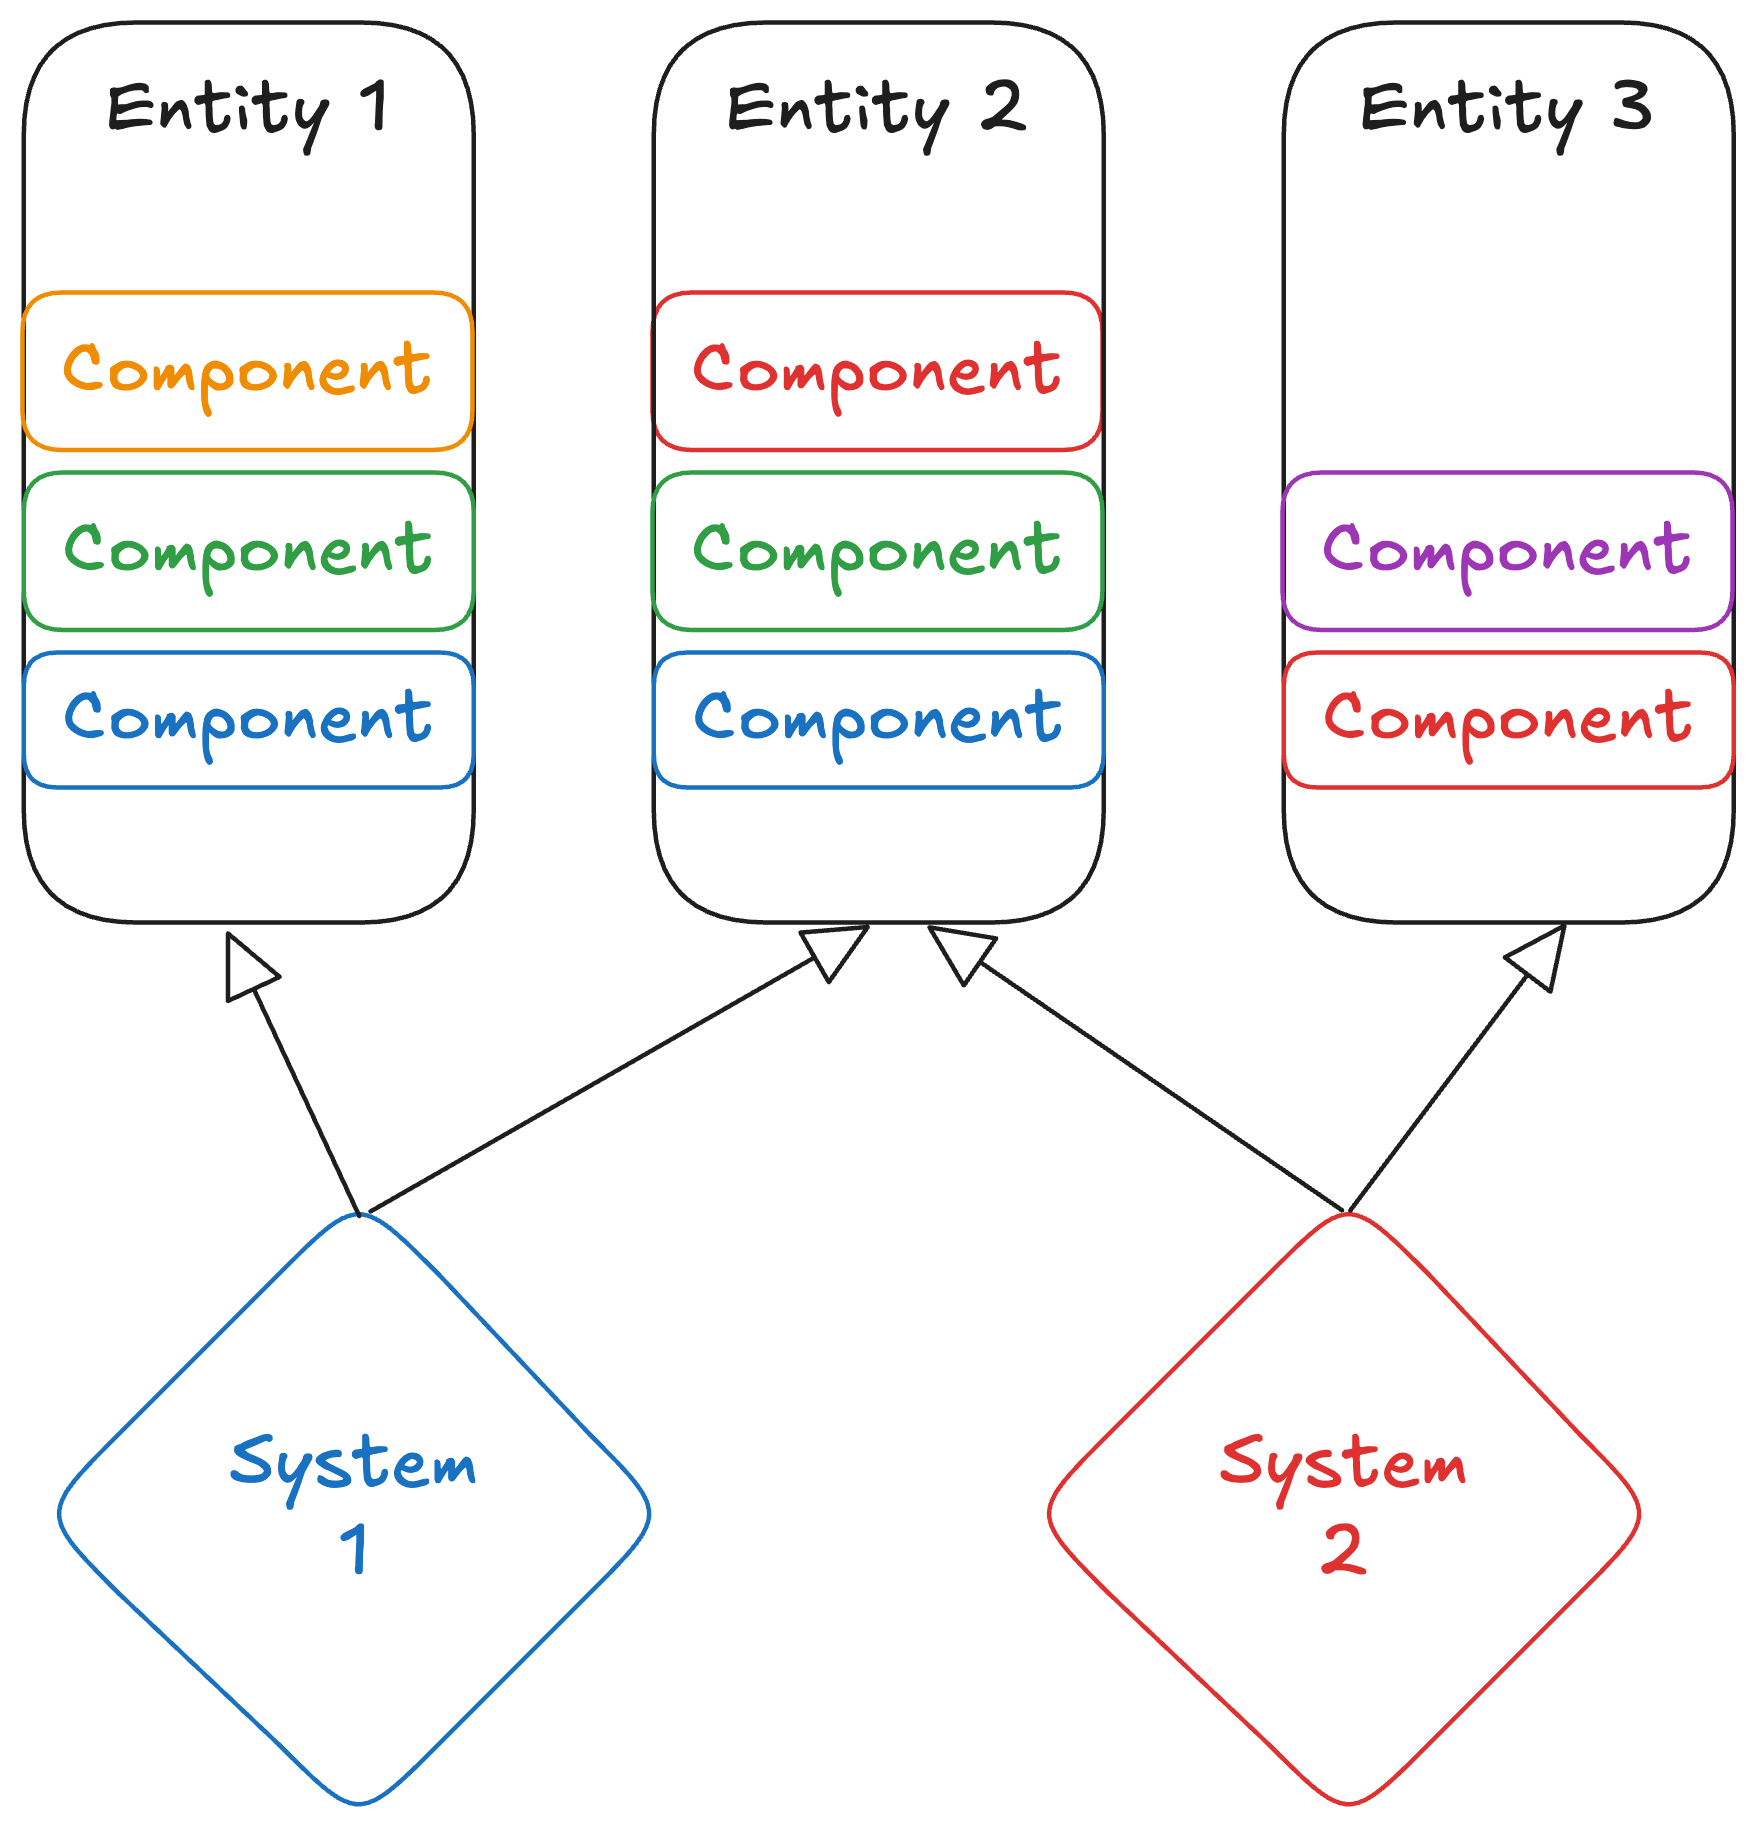
\includegraphics[width=0.3\textwidth]{Chapter4/ECS-visualisatoin.png}
    \caption{ECS visualisation implementation}
    \label{fig:chap-4:ecs-example}
\end{figure}



This choice offered several pros and cons. From the one hand,
the current choice offers flexibility when it comes to drawing
and interacting with shapes on a screen. We wanted to give our
tool and editor-like aesthetic where the user can move the screen and individual
nodes themselves as well as interact with them.
In addition, it is one of the most used libraries in rust for graphic development
and its incorporation with rust implies the ability to take advantage of low level programming.
On the other hand,
this library is still in its early stages, which implies limited documentation
and features. Moreover, as its prioritizes game development, it has a limitation
when dealing with UI concepts and state management. Ultimately, we chose the tool as
the UI is simple enough to not hinder the experience of the tool.

\subsection{Software Testing methodology}
The core philosophy of our testing is Test-Driven-Development. This methodology
was used to develop and validate our critical parts of our code, such as graph validation
or solution enumeration. The main idea of this development is to first write the unit test,
and then develop the code to resolve them. This allows us for the code to be self-documenting
as well as ensuring that we are acting within the expected scope.


Another testing technique that we heavily took advantage of is \textit{Property-based Testing},
which we implement using the \texttt{Proptest} library \footnote{https://github.com/proptest-rs/proptest}.
This idea was inspired by the \texttt{Haskell} library \texttt{QuickCheck}  \cite{claessen_QuickCheckLightweightTool_2000},
where we test the properties of a pure function across a range of inputs. The idea is, the more complex,
the input of the function, the greater is the input space and therefore harder and cumbersome to check all possible
combinations or edge-cases. With \texttt{Proptest}, we check whether a property of our function is
maintained across all possible inputs, such as a sorted output, or a validating assignment.

For our purposes, we use value-based property testing in which:
We define a set of types where in each one we define a \textit{generator} and a \textit{shrinking strategy}.
The \textit{generator} is responsible for generating random values or significant values
that represent the specific type. The \textit{shrinking strategy} is responsible
for finding the smallest case in which our case fails. We then
define test cases that automatically run the generator and shrinker procedures until,
we have tested that our function passes across all generated inputs, or finds the smallest test case it fails on.



\section{Program Visualisation Summary}

The program is composed of a mini UI legend that captures the state and a drawing board.
Contains functionalities as to the current state of the program and the controls to navigate
and operate. Moreover is contains buttons that find solutions
or enumerate through a set of solutions.


%TODO ADD figure
The controls are summarised as follows. We have two main states, which we denote as node state and operation state.
The operation state, determines whether we are adding an edge or a node and the node state determines the type of node that we are adding.
We also provide operations to move nodes around or move the whole canvas around. When in edge mode, we can
click a node to add an edge between to non-homogeneous nodes, where the order implies the direction of the edge.
Moreover, every time you click on a node, you modify its value, so for example for value nodes or for gate nodes you can cycle through
its different types by clicking on them. For each gate, we colour-coded its status, so for example if a gate has an invalid arity,
then its surrounded by a pink circle or if it has an invalid assignment then its coloured red.

For the main algorithms, we provide two metaheuristic algorithms for finding solutions or approximate solutions, using
either evolutionary algorithms or hill climbing search. Moreover for solution enumeration,
we are using a modified backtracking algorithm, which upon execution
returns a list of solutions. We are limiting the algorithm to at most $20$ value nodes
in order to keep the computational expense low. Each time we modify the stucture of the circuit, we reset the solution set.


\section{Solution Selection}

For the solution selection we opted with metaheuristic algorithms. Since these problems are conventionally hard
to find solutions especially as the number of nodes increase, we focused on the idea of approximation
algorithms such in order to find mostly satisfying assingments in large graphs or gadgets.
With the help of the \texttt{genetic\_algorithm}\footnote{https://crates.io/crates/genetic\_algorithm}  library,
we use he \textit{HillClimbing algorithm} and \textit{Evolutionary algorithm}  in order
to find solutions. We will give a brief explanation on how they work in the upcoming sections but in general
we express our graph as a chromosone of \textit{Value} nodes which correspond to nodes in the original graph.
Moreover we formulate our problem as series of gates with references to the location of their
incident value nodes and we count the of unsatisfying gates. The goal of either algorithm
is to minimise the number of errors. Once an assingment is found,
we pass the solutions back into our graph and display them.


\subsection{Hill Climbing Algorithm}

The idea of hill climbing algorithms is to start by some base solution
and repeatedly improve the solution. We allow for $2$ strategies, one
of them strictly always chooses the best neighobur whereas one
allows for stochastic choice. Moreover we allow for additional option
such as multiple re-rurns in order to incaese the odds of finding
a successful assignment.

Overall this algorihtm, one of the simplest and faster algorithms to run and can work
well for convex problems as explained in \cite{schwefel_EvolutionOptimumSeeking_1995}.
It may significantly struggle against large graphs or instances
that multiple changes need to occur in order to reach an optimal point.
In fact we can further argue that hill climbing may struggle on the
\textit{Purify}  gate due to the non-linearity that they present.
Future ideas can adopt \textit{Simulating annealing} which
which is a metaheuristic algorithm, where at the start of our run,
we allow for a greater variance in our choices and as we progress, we become
stricter and stricter with the next neighbour choice \cite{schwefel_EvolutionOptimumSeeking_1995}.

\subsection{Evolutionay Algorithm}

Evolutionary algorithms as the names suggests are based of the
idea of evolution.
They were introduced by \cite{holland_AdaptationNaturalArtificial_1992},
it is a useful algorithm has found several usages in computer science, particularly
in optimisation problems such as \textit{TSP} problems \cite{moon_EfficientGeneticAlgorithm_2002}
or \textit{Neural Networks} \cite{stanley_EvolvingNeuralNetworks_2002,stanley_HypercubeBasedIndirectEncoding_2009}.

Given figure \ref{fig:chap-4:evo-drawing},
we can summarise the 5 core elements of the genetic algorithm:
\begin{enumerate}
    \item \textbf{Chromosones}: Solution assignments of our \textit{PureCircuit} instance.
    \item \textbf{Population}: A set of \textbf{chromosones}.
    \item \textbf{Fitness step}: Evaluation step. We measure how good the assingment is
          by counting the number of errors it has.
    \item \textbf{Selection step}: Given a selection strategy, select
          suitable canditates in order to create the population for the next step.
          In literature, there are many types that one can use \cite{katoch_ReviewGeneticAlgorithm_2021}
          such as \textit{Roulette based} selection, or \textit{Tournament based} selection.
          We mainly use \textit{Tournament based} selection where randomly select a set of
          chrosomones and pick the best one. This process is repeated until enough chromosones have been selected.
    \item \textbf{Crossover step}: Given two chromosones from the
          \textbf{Selection step}, combine the genes from each parent, in order
          to create a new instance. We allow for two main types of crossover methods:
          \begin{enumerate}
              \item \textit{Crossover Uniform}: Each gene of the child is randomly selected from either parent. This allows for
                    diverse solutions to be explored. Can reduce diversity but performs well on large population sizes \cite{katoch_ReviewGeneticAlgorithm_2021}.
              \item \textit{Crossover MultiPoint}: Using figure \ref{fig:chap-4:crossover-cutoff} as reference,
                    we select crossover points that determine cutoff points
                    from each parent. For each even sequence we use the sequence of the other parent. This method
                    can be useful if consecutive pairs of genes are needed to improve the fitness.
          \end{enumerate}
    \item \textbf{Mutation step}: Given the offspring of the
          \textbf{Crossover step}, we stochastically modify each gene in
          order to introduce diversity, which allows our chromosones to explore
          the solution space and escape local optima \cite{katoch_ReviewGeneticAlgorithm_2021}.
\end{enumerate}

\begin{figure}[h!]
    \centering
    \includesvg[width=0.7\textwidth]{Chapter4/intro-1.svg}
    \caption[Visual representation of the genetic algorithm cycle]{Visual representation of the genetic algorithm cycle. Image source \cite{wychowaniec_2021}}
    \label{fig:chap-4:evo-drawing}
\end{figure}


\begin{figure}[h!]
    \centering
    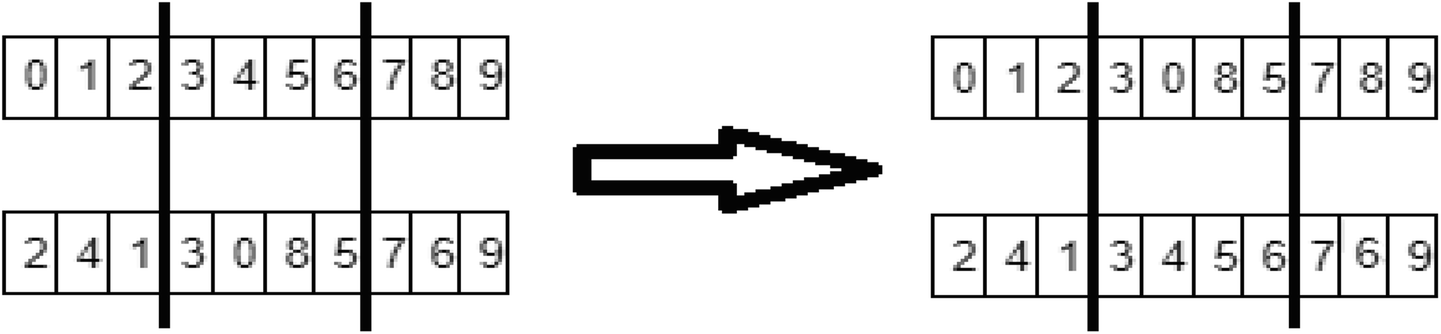
\includegraphics[width=0.3\textwidth]{Chapter4/cutoffpoint.png}
    \caption{Crossover with multiple cutoff points. Image source \cite{katoch_ReviewGeneticAlgorithm_2021}}
    \label{fig:chap-4:crossover-cutoff}
\end{figure}

The repetition of the steps eventually converges to an assignment that is satisfying.
The benefits of these methods over our own personal experimentations is that
it seems to scale significantly well. As we aim for the tool to be usable
for many sitautions, we allow for the user to tune the parameters and stategies to their needs
in order to adapt to each solution.
Moreover, we use speciation techniques were sepearate our chromosones
to different species in order to maintain diversity and increase
the odds of finding a solution.

%%TODO: RECORD STUFF





\subsection{Solution Enumeration}

To enumerate through solutions, we employed a traditional backtracking algorithm. We
split our algorithm to two main procedures:
\textbf{Backtrack Initialisation} and \textbf{Backtrack Solution Enumerator}.



\begin{breakablealgorithm}
    \caption{PureCircuit Backtracking Algorithm Enumerator}
    \begin{algorithmic}
        \Function{BacktrackInstatiation}{pc \texttt{: PureCircuitInstance}}
        \State $V \leftarrow$ \Call{PCExtract}{pc}
        \Comment {Extract value nodes from the \textit{PureCircuit} instance}
        \State $S \leftarrow$ \Call{Arr}{$|V|$, \Call{KleeneSetInit}{$\{0, \bot, 1\}$}}
        \Comment {Create a state vector that contains the \textit{KleeneSet} data-structure.}
        \State $Q \leftarrow$ \Call{PriorityQueueInit}{$\emptyset$}
        \For{$\texttt{el} \in V$}
        \State \texttt{pq\_key} $\leftarrow$ \Call{KeyStruct}{3,  \texttt{el.is\_source}(), \texttt{el.num\_neigh}()}
        \State \Call{PushPQ}{$Q$, \texttt{pq\_key}, \texttt{el.index}}
        \EndFor
        \State \Return $S, Q$
        \EndFunction

        \Function{BacktrackPureCircuit}{pc \texttt{:PureCircuitInstance}}
        \State $S, Q \leftarrow$ \Call{BacktrackInstatiation}{pc}
        \State $A \leftarrow$ \Call{Arr}{$|V|, \emptyset$}
        \State $r \leftarrow$ \Call{BacktrackIteration}{pc, $A$, $S$, $Q$}
        \State \Return $r$
        \EndFunction

        \Function{BacktrackIteration}{
        \Statex \qquad pc \texttt{:PureCircuitInstance},
        \Statex \qquad $A$ \texttt{:Arr[Kleene]},
        \Statex \qquad $S$ \texttt{:Arr[KleeneSet]},
        \Statex \qquad $Q$ \texttt{:PriorityQueue}
        \\}
        \If{\Call{IsEmpty}{$Q$}}
        \State \Return $[A]$
        \EndIf
        \State min\_graph\_ind $\leftarrow$ \Call{ExtractMin}{$Q$}
        \State $r \leftarrow []$
        \For{$v \in S[m]$}
        \State $S' \leftarrow$ \Call{Clone}{$S$}
        \State $Q' \leftarrow$ \Call{Clone}{$Q$}
        \State $A' \leftarrow$ \Call{Clone}{$A$}
        \State $\textit{result} \leftarrow$\Call{UnitPropagate}{\text{pc}, min\_graph\_in, v, $A'$, $S'$, $Q'$}
        \If{$\textit{result} = \bot$}
        \State \textbf{Continue}
        \EndIf
        \State $r' \leftarrow$\Call{BacktrackIteration}{$\text{pc}, A', S', Q'$}
        \State $r \leftarrow$ \Call{ConcatArray}{$r, r'$}
        \EndFor
        \State \Return $r$
        \EndFunction

        \Function{UnitPropagation}{
        \Statex \qquad pc         \texttt{:PureCircuitInstance},
        \Statex \qquad nod\_ind   \texttt{:GraphIndex},
        \Statex \qquad nod\_val   \texttt{:GraphValue},
        \Statex \qquad $A$        \texttt{:Arr[Kleene]},
        \Statex \qquad $S$        \texttt{:Arr[KleeneSet]},
        \Statex \qquad $Q$        \texttt{:PriorityQueue}
        \\}
        \State \Call{AssignNode}{nod\_ind, nod\_val, $A$, $S$, $Q$}
        \State \Call{PropagateNode}{pc, nod\_ind, nod\_val, $A$, $S$, $Q$}
        \While{$\neg$\Call{IsEmpty}{$Q$}$ \wedge$ \Call{PeekKey}{$Q$}.set\_length $=1$}
        \Comment{While the queue contains an element whose value can take only one element, assign its value}
        \State ind $\leftarrow$ \Call{ExtractMin}{$Q$}
        \State val $\leftarrow S[\text{ind}]$
        \State \Call{AssignNode}{ind, val, $A$, $S$, $Q$}
        \State \Call{PropagateNode}{pc, nod\_ind, nod\_val, $A$, $S$, $Q$}
        \EndWhile
        \If {\Call{IsEmpty}{$Q$}}
        \Comment{If every element is assigned, accept}
        \State \Return $\top$
        \EndIf
        \If {\Call{PeekKey}{$Q$}.set\_length $=0$}
        \Comment{If the queue contains an element which does not have a satisfying assignment, discard the current assignment}
        \State \Return $\bot$
        \EndIf
        \State \Return $\top$
        \EndFunction

        \Function{PropagateNode}{
        \Statex \qquad pc         \texttt{:PureCircuitInstance},
        \Statex \qquad nod\_ind   \texttt{:GraphIndex},
        \Statex \qquad $A$        \texttt{:Arr[Kleene]},
        \Statex \qquad $S$        \texttt{:Arr[KleeneSet]},
        \Statex \qquad $Q$        \texttt{:PriorityQueue}
        \\}
        \For{$g \in$ \Call{GetAllGateNeighbours}{pc, nod\_ind}}
        \State $I \leftarrow$ \Call{GetValueSets}{\texttt{Input}}
        \State $O \leftarrow$ \Call{GetValueSets}{\texttt{Output}}
        \State $(I', O') \leftarrow$ \Call{SetSimplification}{$g, I, O$} 
        \Comment{Determine the available value sets for each input output element given the elements that have been already assigned}
        \State \Call{PropagateSetValues}{$Q,S, I', I$}
        \Comment{Propagate the changes to their value sets and to their queue keys for both the input and output elements}
        \State \Call{PropagateSetValues}{$Q,S, O', O$}
        \EndFor
        \EndFunction
    \end{algorithmic}
\end{breakablealgorithm}




\paragraph*{Backtrack Initialisation} We initialise two main structures,
a priority queue $Q$, and a solution map $S$ for each node.
$S$ is the a set of possible values a node can take.
The priority queue will essentially dictate
which nodes to select and evaluate.
We want to reduce the recursive calls as much as possible and eliminate any partial assignments
that lead to unsatisfying solutions.
stores the node references of the value nodes
and uses as keys the structure \textsc{KeyStruct}$(e)$.
The \textsc{KeyStruct} is a structrue that orders elements lexicographically
based on the following order:
\begin{enumerate}
    \item \textbf{In descending}: The number of possible value elements the current node can take
    \item \textbf{In Ascending}: Whether the node has an \textit{in-degree} of $0$
    \item \textbf{In Ascending}: The total number of neighbours
\end{enumerate}
We argue that the above strategy minimises the breadth of the recursive calls. Moreover,
for each node with \textit{in-degree} of $0$ as for each value of their assignment, a solution should exist.
The heurestical argument for this can be observed in Deligkas et al. \cite{deligkas_PureCircuitTightInapproximability_2024}, 
where there construction for finding solutions allows for source nodes to be independent.
Lastly, prioritising nodes with the highest neighbour count implies that we
propagate changes to a greater number gates and therefore maximise the influence of the \textit{Unit Propagation}
procedure.

\paragraph*{Unit Propagation operation}
The algorithm
essentially, assigns the selected value to a node
by modifying to the solution set and the value set.
Then for each gate that is incident to the node apply the \textit{Set simplification}
operation. While the top element of the queue
has one possible solution, extract the solution and repeart the \textit{unit value propagation operation}
until the queue is empty or the cardinality of the value set at the head of the priority queue
is different than $1$. If it's zero then
current assingment is not valid and we return false, otherwise we return true.


\paragraph*{Set simplification operation}
Given a gate, we have a set of possible values for each of our nodes,
as determined by our value set. The idea is
that we want to reduce the set possible values by following the rules of the gate.
For example, we given an \textbf{AND} gate.
If the output value is assigned the value $1$, then we know that the inputs can only take values
$(1,1)$ and therefore we restrict the values of the input sets to $\{1\}, \{1\}$.
If the current solution set of a node is $v_t$, then its updated set is
$v_{t+1} \leftarrow v_t \cap \omega$, where $\omega$ are the set of values denoted
by the simplification operation. We provide the rules of \textbf{AND} and \textbf{OR}
work and in the appendix we provide the full table. %TODO Dont forget this
If a value is not assigned, we denote it as $\cdot$.


\begin{table}[h!]
    \centering
    \begin{tabular}{|c|c|}
        \hline
        \rowcolor[HTML]{EAE1E1}
        {\color[HTML]{333333} \textbf{AND input}}                  & {\color[HTML]{333333} \textbf{Output sets}}                                                  \\ \hline
        $\forall v \in \mathbb{T}: (\cdot, \cdot, v)$              & $(\mathbb{T}_{\geq v},\mathbb{T}_{\geq v}, \{v\} )$                                          \\ \hline
        $\forall v \in \mathbb{T}: (\cdot, v, \cdot)$              & $(\mathbb{T}, \{v\}, \mathbb{T}_{\leq v})$                                                   \\ \hline
        $\forall a,b \in \mathbb{T}: a < b \implies (\cdot, a, b)$ & Invalid combination                                                                          \\ \hline
        $\forall v \in \mathbb{T}: (\cdot, v, v)$                  & $(\mathbb{T}_{\geq v}, \{v\}, \{v\})$                                                        \\ \hline
        $\forall a,b \in \mathbb{T}:a > b \implies (\cdot, a, b)$  & $(\{b\}, \{a\}, \{b\})$                                                                      \\ \hline
        $\forall a,b \in \mathbb{T}: (a, b, \cdot)$                & $(\{a\}, \{b\}, \{\min(a,b) \})$                                                             \\ \hline
        $\forall a,b,c \in \mathbb{T}:  (a, b, c)$                 & $(\{a\}, \{b\}, \{c \})$, only if the triplet $(a,b,c)$ is a correct \textbf{AND} assignment \\ \hline
    \end{tabular}
    \caption{\textbf{AND} value propagation rules}
    \label{tab:chap-4:and-propagation}
\end{table}

\begin{table}[h!]
    \centering
    \begin{tabular}{|c|c|}
        \hline
        \rowcolor[HTML]{EAE1E1}
        {\color[HTML]{333333} \textbf{OR input}}          & {\color[HTML]{333333} \textbf{Output sets}}                                                 \\ \hline
        $\forall v \in \mathbb{T}: (\cdot, \cdot, v)$     & $(\mathbb{T}_{\leq v},\mathbb{T}_{\leq v}, \{v\} )$                                         \\ \hline
        $\forall v \in \mathbb{T}: (\cdot, v, \cdot)$     & $(\mathbb{T}, \{v\}, \mathbb{T}_{\geq v})$                                                  \\ \hline
        $\forall a,b \in \mathbb{T}: a < b (\cdot, a, b)$ & $(\{b\}, \{a\}, \{b\})$                                                                     \\ \hline
        $\forall v \in \mathbb{T}: (\cdot, v, v)$         & $(\mathbb{T}_{\leq v}, \{v\}, \{v\})$                                                       \\ \hline
        $\forall a,b \in \mathbb{T}:a > b (\cdot, a, b)$  & Invalid combination                                                                         \\ \hline
        $\forall a,b \in \mathbb{T}:a > b (a, b, \cdot)$  & $(\{a\}, \{b\}, \{\max(a,b) \})$                                                            \\ \hline
        $\forall a,b,c \in \mathbb{T}:  (a, b, c)$        & $(\{a\}, \{b\}, \{c \})$, only if the triplet $(a,b,c)$ is a correct \textbf{OR} assignment \\ \hline
    \end{tabular}
    \caption{\textbf{OR} value propagation rules}
    \label{tab:chap-4:or-propagation}
\end{table}




\paragraph*{Backtrack Operation}
The \textit{backtrack} operation is summarised in 3 key steps.
If the priority queue is empty then we found a satisfying assignment.
Otherwise, pick a node from the priority queue. For each value in its set,
create a copy of the current queue, current solution assingment and value set state
and apply the \textit{Unit value propagation} operation. After that create a recursive call
apply the \textit{backtrack opertation} again until the current recursion chain
terminates with a solution or rejects.
At the root of every execution call, merge the solution assignments in each level and return
the sets. The root call will return a set of every possible valid assingment set.


\subsubsection{Correctness and Running Time analysis}

For the running time analysis, we can observe that each time we assign a node,
the unit propagation operation, resticts the solution set of the value nodes that are incident
by one gate. Even in the worst case scenario where no reduction occurs, we can clearly
see that each time, our priority queue will select a node and will recurse through each of its possible values,
creating a call tree with depth of at most $n$. Therefore we can argue that the running time of the algorithm
is $O(3^n)$, we can observe as the unit propagation and set reduction methods attempt to reduce in the average cases.


As for correctness, the algorithm essentially picks nodes in a certain order and selects a
value that we believe that will give a satisfying assignment. We only have to look
at what happens at the \textit{unit propagation} stage. We can observe that in each stage,
we are essentially limiting the set of solutions to only the ones
that will give a satisfying assignment. The idea is that we are fast-forwarding the backtracking calls
by taking advantage of the localised changes of each gate.
Value that we discard are nodes that are guarnteed to give unsatisfying assingments and therefore
we are not discrading any solutions.
If the value set of a node is zero, it means that no assignment
will lead to a solution and therefore we reject the current path.
If no nodes are left in the queue, that means that all value nodes are assigned and therefore we can return the current assignment.
This implies that our resulting array of assignments contains only valid solutions, and this array
covers the maximal solution set.


\subsection{Future Extensions}

\subsubsection{Algorithmic Extensions}
Although the aforementioned algorithms work as expected, there are several improvements that can be made.
For all three of the algoritmic methods we mentioned, the first and most important extension
is to treat weakly directly connected components individually. Trivially an assignment in one
weakly connected component should not affect the solution set of the other one.
We can therefore reduce the search spaces of our problems by finding
the solution sets in each graph seperately. Moreover for the
\textit{backtracking} algorithm, we can extend the above idea by considering
the cartesian product of the solution sets, meaning:
let $G_i$ denote a (weakly) connected component of $G$ and $\textbf{sol}(\cdot)$
denotes its solution set. Its trivial to observe that
$$
    \textbf{sol}(G) = \bigtimes_{k \in [k]}  \textbf{sol}(G_k)
$$

We can also optimise the backtracking algorithm even further.
First one can observe that if our graph was acyclic, then
the permutation of the nodes with no \textit{in-degree} solutions essentially
dictate the assignments of the downstream nodes (excluding nodes incident
to purify gates). With this in mind, we can apply the following sequence
of steps to make the backtracking algorithm simpler:
\begin{enumerate}
    \item Identify the strongly connected components (SCCs) of the circuit, using polynomial
          time algorithms such as Kosaraju's Algorithm \cite{sharir_StrongconnectivityAlgorithmIts_1981} 
          or Gabow's Algorithm \cite{gabow_PathbasedDepthfirstSearch_2000}. 
    \item Treating SCCs as an individual node, identify nodes by their distances from
          base nodes (nodes with no incoming edges)
    \item Extend the backtracking algorithm so instead of the using the is start label,
          use the distance from base instead. The greater distance a node has from the
          base, the less impact it has and therefore should be postponed in later stages of the
          backtracking calls.
\end{enumerate}

We argue that the above heuristic may result in improved average times but of course
further research can be done in order to determine more suitable selection heuristics.
Furthermore, an additional heuristic that we failed to consider is using the notion
of alternation or varying path.
This has been introduced by \cite{eichelberger_HazardDetectionCombinational_1965}
and the idea is the ``application'' of the gates to propagate values.
Their algorithm can be summarised as such:
Start with an initial set of nodes, and apply gates of each circuit enough times.
For nodes that alternate their values between $0,1$, replace their value with $\bot$
Repeat until no altrenation occurs. This algorithm is still exponential
in its running time but one could deduce useful insights as to notion
of alternating paths.
It has to be noted that it may not be entirely clear how such construction
could be applied as the purify gate has a non-deterministic output, meaning
for the $\bot$ value, the outputs could be multiple.
